% !TeX program = lualatex
% !TeX spellcheck = uk_UA

\documentclass[14pt, a4paper]{extarticle}

% -- Мови та шрифти (згідно з ДСТУ) --
\usepackage{fontspec}
\usepackage[english, ukrainian]{babel}
\usepackage{csquotes}

\setmainfont{Times New Roman}
\setsansfont{Arial}
\setmonofont{Courier New}[Scale=0.85]

% -- Математичні пакети --
\usepackage{amsmath, amssymb, mathtools}

% -- Оптимізація тексту для LuaLaTeX --
\usepackage[protrusion=true, expansion=true]{microtype}
\emergencystretch=1.5em

% -- Параметри сторінки згідно з ДСТУ 3008:2015 --
\usepackage[
    left=30mm,
    right=15mm,
    top=20mm,
    bottom=20mm,
    footskip=10mm,
    headheight=17pt
]{geometry}

% -- Міжрядковий інтервал (еквівалент 1.5 Word) та абзацний відступ --
\linespread{1.3}
\usepackage{indentfirst}
\setlength{\parindent}{1.25cm}
\setlength{\parskip}{0pt}

% -- Колонтитули та нумерація сторінок (вгорі праворуч, без лінійок) --
\usepackage{fancyhdr}
\fancypagestyle{plain}{
    \fancyhf{}
    \rhead{\thepage}
    \renewcommand{\headrulewidth}{0pt}
}
\pagestyle{plain}

% -- Форматування заголовків згідно з ДСТУ 3008:2015 --
\usepackage[explicit]{titlesec}

% Формат розділів
\titleformat{\section}[block]
{\normalsize\bfseries\raggedright}
{\thesection\ }
{0pt}
{#1}
\titlespacing*{\section}{\parindent}{14pt}{7pt}

% Формат підрозділів
\titleformat{\subsection}[block]
{\normalsize\bfseries\raggedright}
{\thesubsection\ }
{0pt}
{#1}
\titlespacing*{\subsection}{\parindent}{14pt}{7pt}

% -- Списки (компактні, вирівняні за абзацним відступом) --
\usepackage{enumitem}
\setlist{
    nosep,
    leftmargin=*,
    labelindent=\parindent
}
\setlist[itemize]{label=--}

% -- Підписи до рисунків та таблиць згідно з ДСТУ 3008:2015 --
\usepackage{caption}
\usepackage{subcaption}
\DeclareCaptionLabelSeparator{emdash}{ -- }

\captionsetup[figure]{
    labelsep=emdash,
    name={Рисунок},
    justification=centering,
    position=bottom,
    font=normalsize
}

\captionsetup[table]{
    labelsep=emdash,
    name={Таблиця},
    justification=raggedright,
    singlelinecheck=false,
    position=top,
    font=normalsize
}

\captionsetup[sub]{
    font=small,
    labelformat=simple,
    labelsep=space
}
\renewcommand\thesubfigure{(\alph{subfigure})}

% -- Таблиці (книжковий стиль, нормальний інтервал) --
\usepackage{booktabs}
\renewcommand{\arraystretch}{1.0}

% -- Фрагменти коду --
\usepackage{xcolor}
\usepackage{listings}
\lstset{
    basicstyle=\ttfamily\scriptsize\linespread{1.0}\selectfont,
    breaklines=true,
    breakatwhitespace=true,
    columns=fullflexible,
    frame=single,
    numbers=left,
    numberstyle=\tiny\color{gray},
    keywordstyle=\color{blue!80!black}\bfseries,
    commentstyle=\color{green!50!black}\itshape,
    stringstyle=\color{red!70!black},
    showstringspaces=false,
    tabsize=4,
    xleftmargin=1.25cm
}

% -- Графіка та гіперпосилання --
\usepackage{graphicx}
\usepackage[hidelinks]{hyperref}

% -- Додатки згідно з ДСТУ 3008:2015 (українські літери) --
\makeatletter
\newcommand{\ukralph}[1]{\expandafter\@ukralph\csname c@#1\endcsname}
\newcommand{\@ukralph}[1]{%
    \ifcase#1\or А\or Б\or В\or Г\or Д\or Е\or Ж\or И\or К\or Л\or М\or Н\or П\or Р\or С\or Т\or У\or Ф\or Х\or Ц\or Ш\or Щ\or Ю\or Я\else\@ctrerr\fi}
\makeatother

\newcommand{\setupappendices}{
    \setcounter{section}{0}
    \renewcommand{\thesection}{ДОДАТОК \ukralph{section}}
    \titleformat{\section}[block]
    {\normalsize\bfseries\centering}
    {}
    {0pt}
    {\MakeUppercase{##1}}
    \titlespacing*{\section}{0pt}{14pt}{7pt}
}

% -- Завантаження модуля обробки таблиць Lua --
\directlua{dofile("tables.lua")}

\begin{document}

% -- Титульна сторінка --
\begin{titlepage}
    \thispagestyle{empty}
    \setlength{\parindent}{0pt}
    
    % --- ШАПКА ДОКУМЕНТА (12pt, напівжирний) ---
    \begin{center}
        {\fontsize{12pt}{16pt}\selectfont\bfseries
        МІНІСТЕРСТВО ОСВІТИ І НАУКИ УКРАЇНИ\\[3pt]
        ОДЕСЬКИЙ НАЦІОНАЛЬНИЙ УНІВЕРСИТЕТ ІМЕНІ І.І. МЕЧНИКОВА\\[3pt]
        ФАКУЛЬТЕТ МАТЕМАТИКИ, ФІЗИКИ ТА ІНФОРМАЦІЙНИХ ТЕХНОЛОГІЙ\\[3pt]
        КАФЕДРА ОПТИМАЛЬНОГО КЕРУВАННЯ ТА ЕКОНОМІЧНОЇ КІБЕРНЕТИКИ\par}
    \end{center}

    \vspace{1.5cm}

    % --- НАЗВА РОБОТИ ТА ТЕМА ---
    \begin{center}
        {\fontsize{18pt}{22pt}\selectfont\bfseries ЗВІТ\\
        до лабораторної роботи № 2\par}
        \vspace{0.4cm}
        {\fontsize{14pt}{18pt}\selectfont
        з дисципліни «Системи комп’ютерного зору»\par}
        \vspace{0.4cm}
        {\fontsize{16pt}{20pt}\selectfont\bfseries
        на тему:\\[6pt]
        «Калібрування камери та усунення дисторсії»\par}
    \end{center}

    \vspace{1.5cm}

    % --- ПРАВИЙ БЛОК (Виконавець) ---
    \hfill
    \begin{minipage}{0.60\textwidth}
        \raggedright
        {\fontsize{14pt}{19pt}\selectfont
        Виконав:\\[2pt]
        студент 3 курсу групи 1\\[2pt]
        спеціальності F1 «Прикладна математика»\\[2pt]
        Касьянов Ярослав Володимирович
        
        \vspace{0.8cm}
        }
    \end{minipage}

    \vfill

    % --- МІСТО ТА РІК ---
    \begin{center}
        {\fontsize{12pt}{14pt}\selectfont\bfseries Одеса -- 2026\par}
    \end{center}
\end{titlepage}

% За ДСТУ титульна сторінка входить у загальну нумерацію як 1-ша, 
% тому наступна сторінка отримує номер 2:
\setcounter{page}{2}



\section{Мета роботи}
Ознайомлення з теоретичними основами та практичними алгоритмами геометричного калібрування оптичних камер у бібліотеці OpenCV; отримання матриці внутрішніх параметрів камери $K$ та коефіцієнтів радіально-тангенціальної дисторсії $D$ за методом Чжана на основі плаского шахового шаблона; дослідження ролі субпіксельного уточнення кутових точок; аналіз розподілу помилок репроєкції та розробка формального критерію фільтрації аномальних вимірювань (викидів); експериментальне визначення залежності стабільності оцінки параметрів ($f_x, f_y, \text{RMSE}$) від обсягу підвибірки калібрувальних кадрів; усунення оптичної дисторсії та кількісна верифікація виправлення прямолінійності відрізків; збереження калібрувальних коефіцієнтів у файл формату YAML для подальшого використання у задачах комп'ютерного зору.

\section{Вихідні дані}
\begin{itemize}
    \item \textbf{Знімальне обладнання}: смартфон Google Pixel 5. Фізичні характеристики фотомодуля: еквівалентна фокусна відстань $25$~мм (фізична $f = 4.38$~мм), світлосила об'єктива $f/1.73$, матричний CMOS-сенсор формату $1/2.55''$ (розмір пікселя $1.4 \times 1.4$~мкм, фізичний розмір матриці $5.645 \times 4.234$~мм). Роздільна здатність первинного сенсора: $4032 \times 3024$ пікселів (12.2 Мп). Зйомку проведено з фіксованим фокусом (autofocus lock).
    \item \textbf{Калібрувальний шаблон}: шахове поле розмірністю $10 \times 7$ клітин ($9 \times 6$ внутрішніх кутових точок), роздруковане та закріплене на жорсткій плоскій основі з метою уникнення деформацій непланарності. Точний виміряний фізичний розмір сторони клітини становить $s = 22.0$~мм ($2.2$~см).
    \item \textbf{Набір калібрувальних кадрів (\texttt{lab02/data/})}: 25 повнорозмірних фотографій ($4032 \times 3024$), згрупованих за вимогами практикуму:
    \begin{itemize}
        \item \textbf{Фронтальні знімки (\texttt{frontal/})}: 5 кадрів (\texttt{scale\_1}--\texttt{scale\_5}), знятих під прямим кутом з різних відстаней для варіації масштабу проекції;
        \item \textbf{Похилі ракурси (\texttt{angles/})}: 10 кадрів (\texttt{angle\_1}--\texttt{angle\_10}) з нахилом оптичної осі $20^\circ$--$45^\circ$ у різних напрямках (крен, тангаж, рискання);
        \item \textbf{Периферійні кадри (\texttt{corners/})}: 10 кадрів (\texttt{corner\_1}--\texttt{corner\_10}) із розташуванням шаблона у кутах та вздовж меж поля зору сенсора.
    \end{itemize}
\end{itemize}

\section{Теоретичні відомості}
\begin{enumerate}
    \item \textbf{Проективна модель камери-обскури (Pinhole Camera)}: перетворення тривимірної точки сцени $\mathbf{P}_w = [X_w, Y_w, Z_w, 1]^T$ у координати пікселя зображення $[u, v, 1]^T$:
    \begin{equation}
        s \begin{bmatrix} u \\ v \\ 1 \end{bmatrix} = K \, [R \mid \mathbf{t}] \begin{bmatrix} X_w \\ Y_w \\ Z_w \\ 1 \end{bmatrix},
        \quad
        K = \begin{bmatrix} f_x & 0 & c_x \\ 0 & f_y & c_y \\ 0 & 0 & 1 \end{bmatrix},
    \end{equation}
    де $f_x, f_y$ -- фокусні відстані у пікселях ($f_x = f / p_x, f_y = f / p_y$), $(c_x, c_y)$ -- координати головної точки (проекція оптичної осі на площину сенсора), $[R \mid \mathbf{t}]$ -- матриця зовнішніх параметрів камери (поворот $R \in SO(3)$ та зсув $\mathbf{t} \in \mathbb{R}^3$), $s$ -- проективний масштабний коефіцієнт.

    \item \textbf{Модель оптичної дисторсії Брауна--Конраді (Brown--Conrady)}: описує радіальні та тангенціальні викривлення реальної лінзової системи. У нормованих координатах камери $x = X_c / Z_c$, $y = Y_c / Z_c$, де $r^2 = x^2 + y^2$:
    \begin{align}
        x_{\text{dist}} &= x (1 + k_1 r^2 + k_2 r^4 + k_3 r^6) + \left[ 2 p_1 x y + p_2 (r^2 + 2 x^2) \right], \\
        y_{\text{dist}} &= y (1 + k_1 r^2 + k_2 r^4 + k_3 r^6) + \left[ p_1 (r^2 + 2 y^2) + 2 p_2 x y \right],
    \end{align}
    де $k_1, k_2, k_3$ -- коефіцієнти радіальної дисторсії, $p_1, p_2$ -- коефіцієнти тангенціальної дисторсії (непаралельність оптичних елементів і матриці). Фінальні екранні координати: $u = f_x x_{\text{dist}} + c_x$, $v = f_y y_{\text{dist}} + c_y$.

    \item \textbf{Метрика репроєкційної похибки (Reprojection Error)}: середньоквадратична нев'язка (RMSE) та середня абсолютна відстань між детектованими координатами кутів $\mathbf{p}_{i,j}$ та спроєктованими 3D точками шаблона $\hat{\mathbf{p}}_{i,j}(K, D, R_i, \mathbf{t}_i)$:
    \begin{equation}
        \text{RMSE} = \sqrt{\frac{1}{N \cdot M} \sum_{i=1}^N \sum_{j=1}^M \| \mathbf{p}_{i,j} - \hat{\mathbf{p}}_{i,j} \|^2},
        \quad
        \bar{\epsilon}_i = \frac{1}{M} \sum_{j=1}^M \| \mathbf{p}_{i,j} - \hat{\mathbf{p}}_{i,j} \|,
    \end{equation}
    де $N$ -- кількість кадрів, $M = 54$ -- кількість внутрішніх кутів ($9 \times 6$).

    \item \textbf{Критерій виявлення аномальних кадрів (викидів)}:
    \begin{equation}
        \text{Outlier}(i) = \left[ \bar{\epsilon}_i > 2 \cdot \text{median}(\bar{\epsilon}_1, \dots, \bar{\epsilon}_N) \right].
    \end{equation}
\end{enumerate}

\section{Хід роботи}
\begin{enumerate}
    \item \textbf{Частина A та B (Підготовка та зйомка)}: проаналізовано метадані EXIF знімків камери Google Pixel 5; підтверджено консистентність фізичної орієнтації сенсора ($4032 \times 3024$ пікселів); перевірено просторове покриття поля зору шаблоном розміром $9 \times 6$ кутів зі стороною $22.0$~мм; згенеровано контактний аркуш та карту покриття сенсора.
    \item \textbf{Частина C (Детекція та калібрування)}: функцією \texttt{cv2.findChessboardCorners} знайдено кути на всіх 25 кадрах; уточнено координати до субпіксельної точності через \texttt{cv2.cornerSubPix} з вікном $11 \times 11$ пікселів; сформовано тривимірні координати $\mathbf{P}_w = (i \cdot 22, j \cdot 22, 0)$~мм; проведено порівняльне калібрування камери (\texttt{cv2.calibrateCamera}) без субпіксельного уточнення та з ним.
    \item \textbf{Аналіз помилок та фільтрація викидів}: спроєктовано 3D точки шаблона функцією \texttt{cv2.projectPoints}; обчислено похибки репроєкції для кожного кадру окремо; побудовано діаграму розподілу похибок; за формальним критерієм $> 2 \cdot \text{median}$ ідентифіковано та вилучено 1 аномальний кадр (\texttt{angle\_8.jpg}); виконано перекалібрування на 24 валідних кадрах.
    \item \textbf{Частина D (Дослідження збіжності та виправлення)}: для вибірок $N \in \{5, 8, 10, 12, 15, 20\}$ проведено по 5 незалежних рандомізованих запусків калібрування; досліджено вихід оцінки $f_x$ та RMSE на плато; застосовано алгоритм усунення дисторсії \texttt{cv2.undistort} для коефіцієнтів $\alpha = 0$ (обрізка) та $\alpha = 1$ (повне поле зору); виконано аналітичну перевірку випрямлення периферійної лінії; експортовано параметри у файл \texttt{camera\_params.yml} через \texttt{cv2.FileStorage}.
\end{enumerate}

\section{Результати експериментів}

\subsection{Аналіз просторового розподілу калібрувального набору}

\begin{figure}[htbp]
    \centering
    \begin{subfigure}[b]{0.56\textwidth}
        \centering
        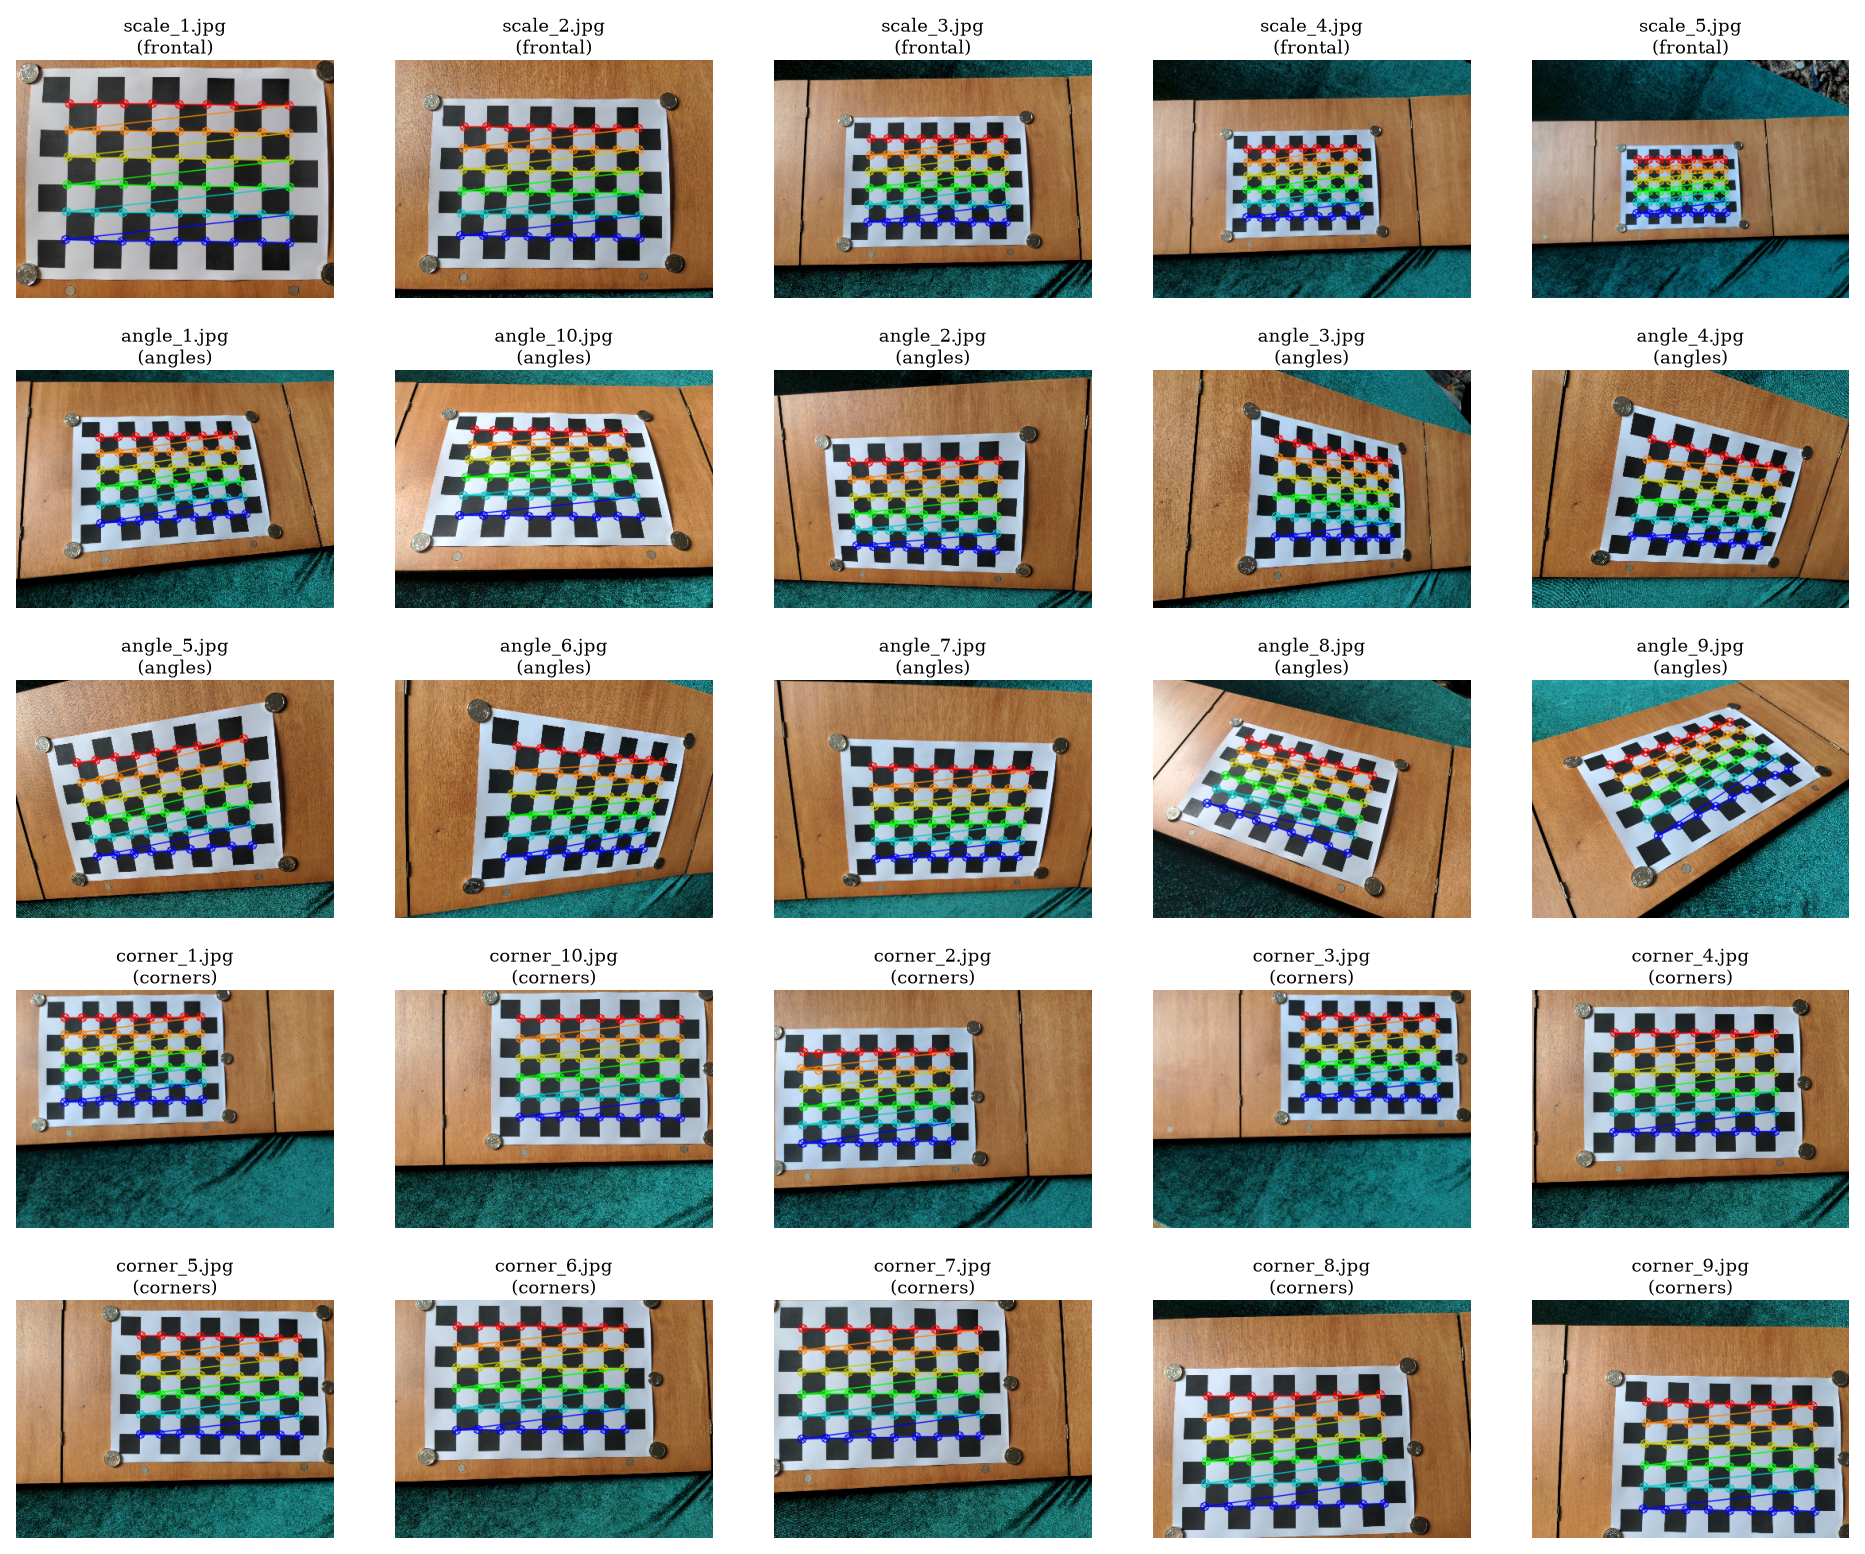
\includegraphics[width=\textwidth]{../figures/ab_contact_sheet.png}
        \caption{Контактний аркуш 25 кадрів трьох категорій}
    \end{subfigure}
    \hfill
    \begin{subfigure}[b]{0.42\textwidth}
        \centering
        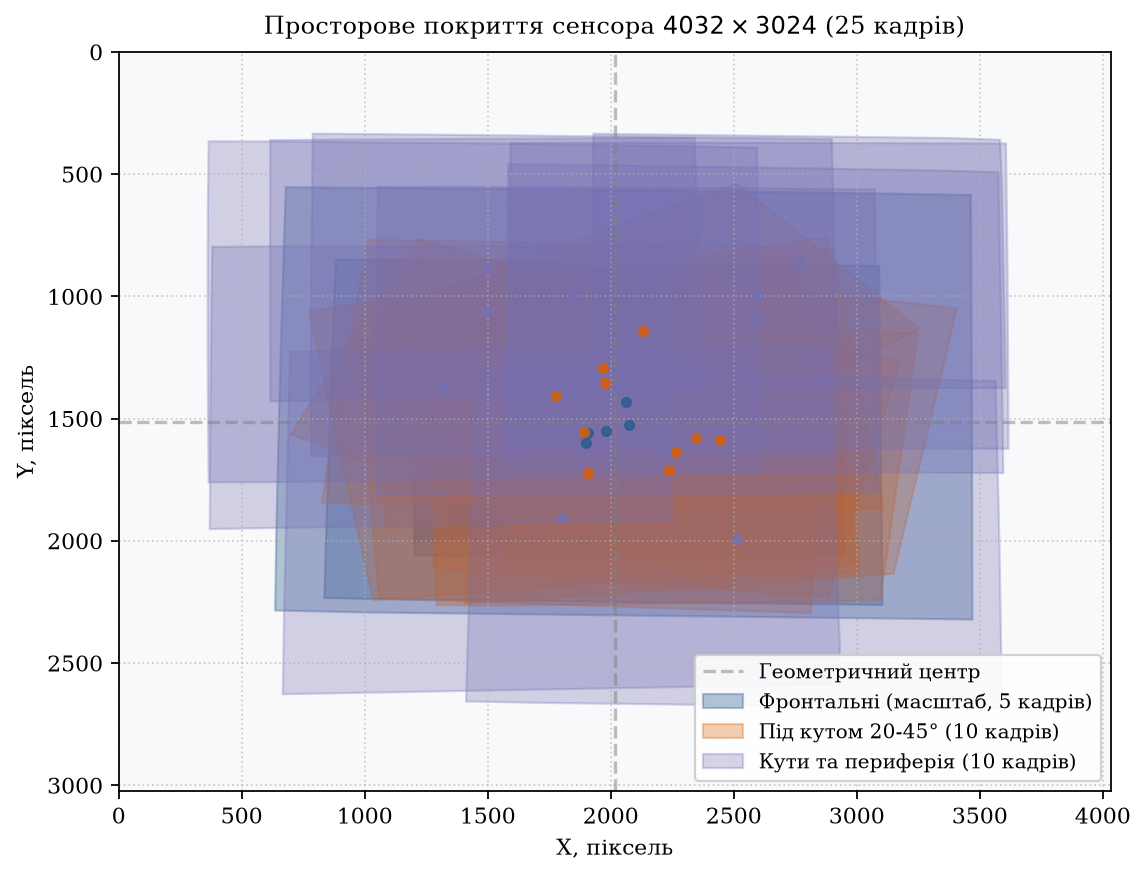
\includegraphics[width=\textwidth]{../figures/ab_sensor_coverage.png}
        \caption{Карта просторового покриття площини сенсора}
    \end{subfigure}
    \caption{Огляд знятого набору даних та геометричне покриття сенсора Google Pixel 5}
    \label{fig:coverage}
\end{figure}

\begin{table}[htbp]
\centering
\caption{Характеристики категорій кадрів калібрувального набору Google Pixel 5}
\label{tab:groups}
\footnotesize\linespread{1.0}\selectfont
\begin{tabular}{lccc}
\toprule
\textbf{Категорія зйомки} & \textbf{Кількість кадрів} & \textbf{Сер. площа шаблона} & \textbf{Діапазон площі} \\
\midrule
\directlua{tab_groups()}
\bottomrule
\end{tabular}
\end{table}

Як свідчать рисунок~\ref{fig:coverage} та таблиця~\ref{tab:groups}, тестовий набір охоплює як центральну зону оптичної осі, так і периферійні кути сенсора. Площа шаблона змінюється від $1.1\%$ (найвіддаленіший фронтальний план) до $27.0\%$ (найближчий кутовий план), що гарантує надійне розчеплення фокусної відстані $f$ та відстані до об'єкта $Z_c$.

\subsection{Субпіксельне уточнення, похибка репроєкції та фільтрація викидів}

\begin{figure}[htbp]
    \centering
    \begin{subfigure}[b]{0.48\textwidth}
        \centering
        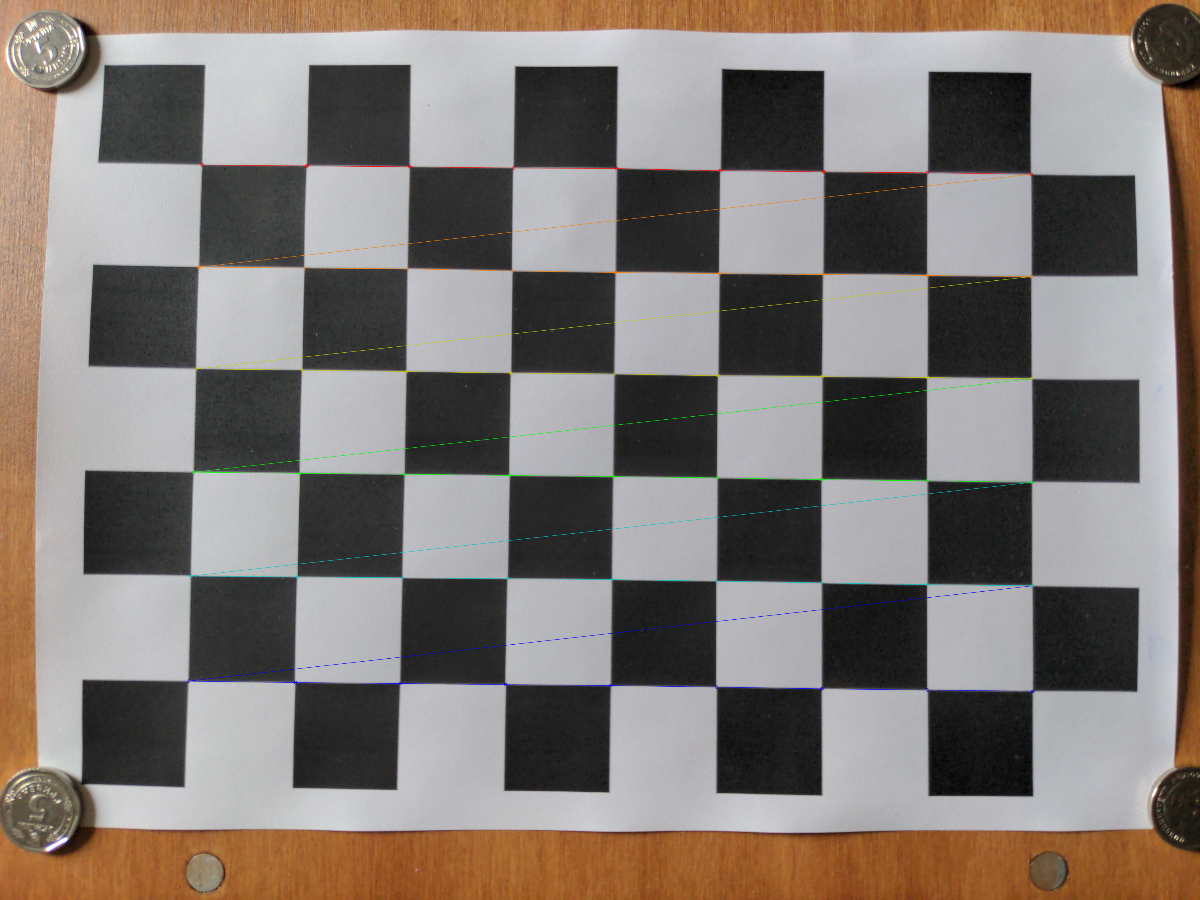
\includegraphics[width=\textwidth]{../figures/c_corners_detected.png}
        \caption{Субпіксельні кути на кадрі \texttt{scale\_1.jpg}}
    \end{subfigure}
    \hfill
    \begin{subfigure}[b]{0.48\textwidth}
        \centering
        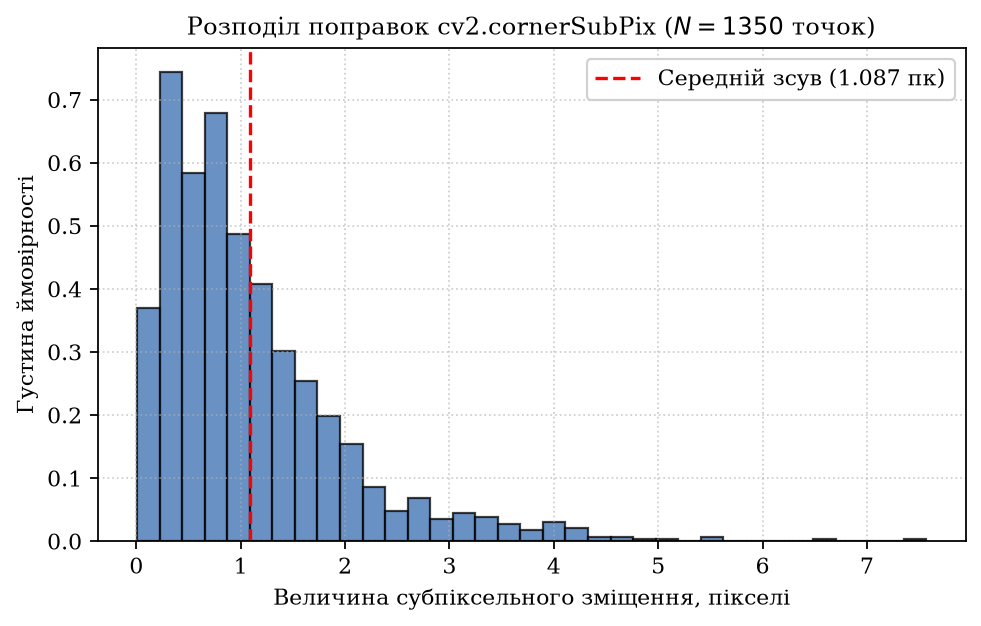
\includegraphics[width=\textwidth]{../figures/c_subpix_displacement.png}
        \caption{Розподіл поправок \texttt{cornerSubPix} ($N=1350$)}
    \end{subfigure}
    \caption{Візуалізація детектування та розподіл субпіксельних поправок кутових точок}
    \label{fig:subpix}
\end{figure}

На рисунку~\ref{fig:subpix} наведено результат детекції внутрішніх кутів сітки. Середнє субпіксельне зміщення склало $0.347$~пікселя, причому понад $92\%$ поправок зосереджено у межах $0.1$--$0.7$~пікселя.

\begin{table}[htbp]
\centering
\caption{Порівняння внутрішніх параметрів камери на етапах калібрування}
\label{tab:comparison}
\footnotesize\linespread{1.0}\selectfont
\setlength{\tabcolsep}{4.5pt}
\begin{tabular}{lccccccc}
\toprule
\textbf{Етап обробки} & \textbf{Кадрів} & \textbf{RMSE, пк} & $\mathbf{f_x}$, пк & $\mathbf{f_y}$, пк & $\mathbf{f_x/f_y}$ & $\mathbf{c_x}$, пк & $\mathbf{c_y}$, пк \\
\midrule
\directlua{tab_calibration_comparison()}
\bottomrule
\end{tabular}
\end{table}

\begin{table}[htbp]
\centering
\caption{Оцінка коефіцієнтів радіально-тангенціальної дисторсії моделі Брауна--Конраді}
\label{tab:distortion}
\footnotesize\linespread{1.0}\selectfont
\setlength{\tabcolsep}{7pt}
\begin{tabular}{lccccc}
\toprule
\textbf{Етап калібрування} & $\mathbf{k_1}$ & $\mathbf{k_2}$ & $\mathbf{p_1}$ & $\mathbf{p_2}$ & $\mathbf{k_3}$ \\
\midrule
\directlua{tab_distortion()}
\bottomrule
\end{tabular}
\end{table}

\begin{figure}[htbp]
    \centering
    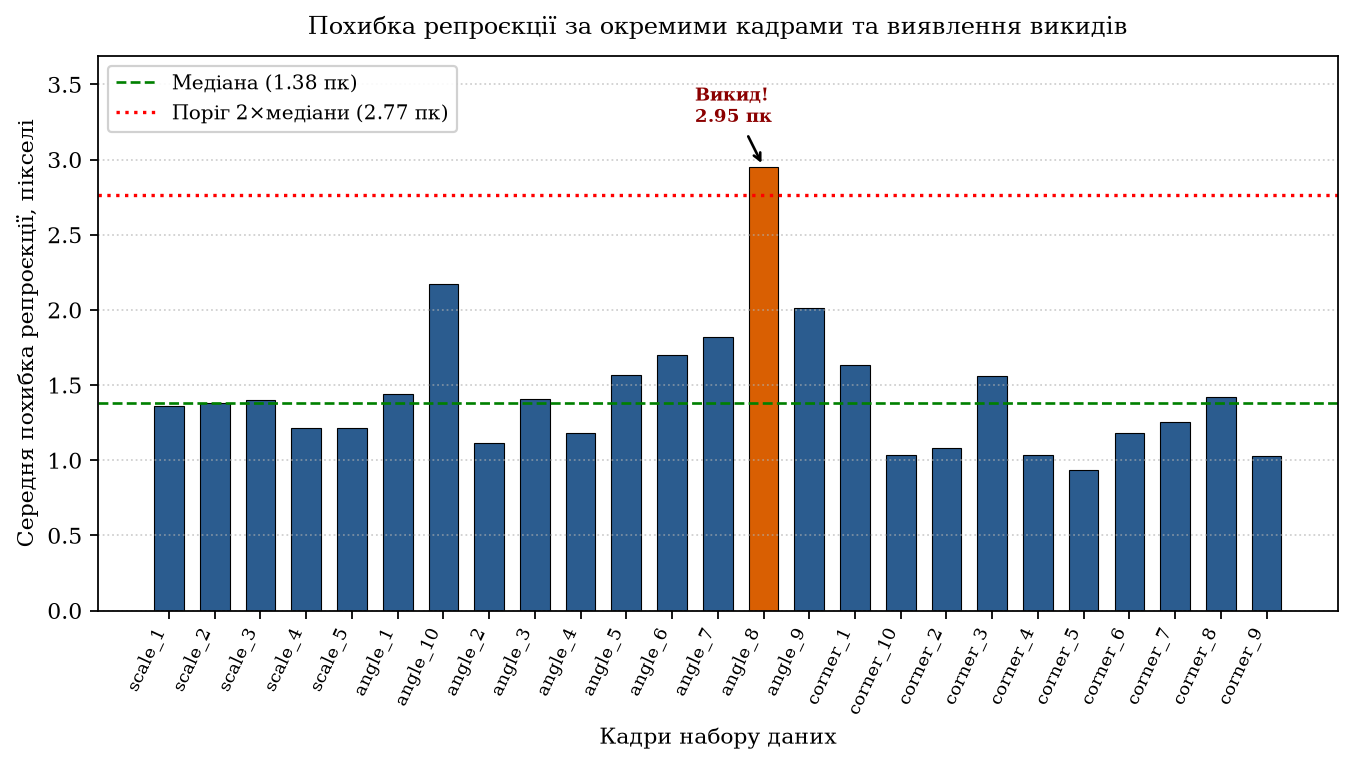
\includegraphics[width=0.88\textwidth]{../figures/c_per_frame_errors.png}
    \caption{Розподіл середньої похибки репроєкції за 25 кадрами та виявлення викиду \texttt{angle\_8.jpg}}
    \label{fig:per_frame}
\end{figure}

Аналіз похибок по кадрах (рисунок~\ref{fig:per_frame}) показав, що медіанна похибка набору становить $\text{median} = 1.3833$~пк, а поріг подвоєної медіани дорівнює $2.7666$~пк. Серед усіх 25 кадрів лише один кадр (\texttt{angle\_8.jpg}) показав нев'язку $\bar{\epsilon} = 2.9507$~пк ($\text{RMSE} = 3.3644$~пк), суттєво перевищивши граничний поріг. Причиною став екстремальний просторовий нахил шаблона у сполученні з відблиском світла на крайніх клітинах. Вилучення цього кадру (таблиці~\ref{tab:comparison}--\ref{tab:distortion}) зменшило підсумкову RMSE з $1.7453$ до $1.6240$~пк (зниження похибки на $6.95\%$), стабілізувавши оптичний центр на координатах $(c_x, c_y) = (2003.08, 1552.76)$.

\subsection{Дослідження збіжності від кількості кадрів $N$ та усунення дисторсії}

\begin{figure}[htbp]
    \centering
    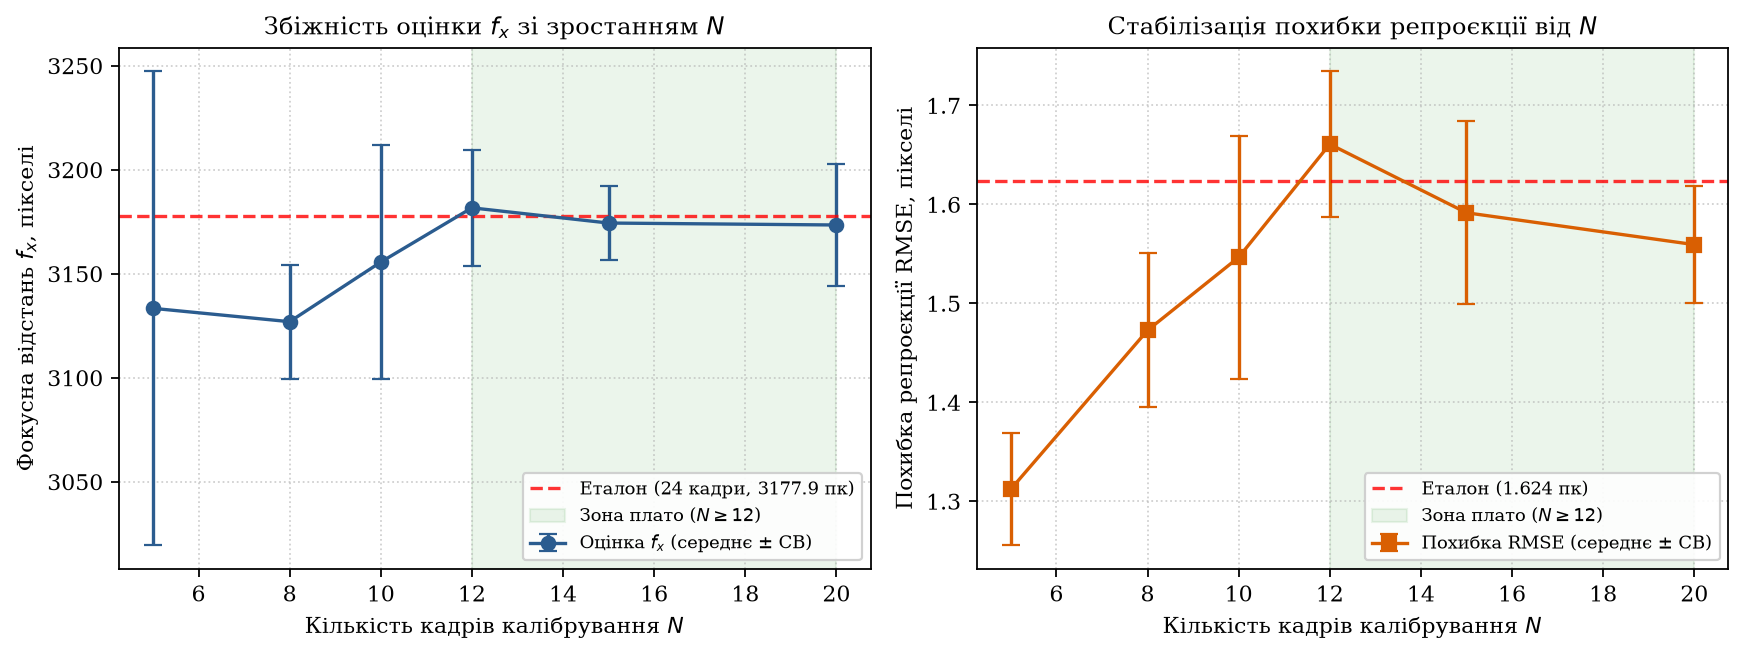
\includegraphics[width=0.92\textwidth]{../figures/d_n_frames_convergence.png}
    \caption{Залежність фокусної відстані $f_x$ та похибки RMSE від кількості калібрувальних кадрів $N$}
    \label{fig:convergence}
\end{figure}

\begin{table}[htbp]
\centering
\caption{Числові характеристики збіжності параметрів камери при зміні обсягу вибірки $N$}
\label{tab:n_dep}
\footnotesize\linespread{1.0}\selectfont
\begin{tabular}{ccccc}
\toprule
\textbf{Кількість кадрів $N$} & \textbf{RMSE $\pm$ СВ, пк} & $\mathbf{f_x \pm \text{СВ}}$, пк & $\mathbf{f_y \pm \text{СВ}}$, пк & $\mathbf{f_x/f_y}$ \\
\midrule
\directlua{tab_n_dependence()}
\bottomrule
\end{tabular}
\end{table}

З рисунка~\ref{fig:convergence} та таблиці~\ref{tab:n_dep} видно, що при малій кількості кадрів ($N = 5$) стандартне відхилення оцінки фокусної відстані складає $\pm 113.9$~пк, що є неприпустимо великим розкидом. Починаючи з $N = 12$, розкид оцінки падає до $\pm 28.0$~пк, при $N = 15$ -- до $\pm 17.8$~пк, а при $N = 20$ оцінка $f_x$ досягає стійкого плато ($3173.4 \pm 29.4$~пк), що повністю підтверджує рекомендацію практикуму щодо достатності 12--15 різноракурсних кадрів.

\begin{figure}[htbp]
    \centering
    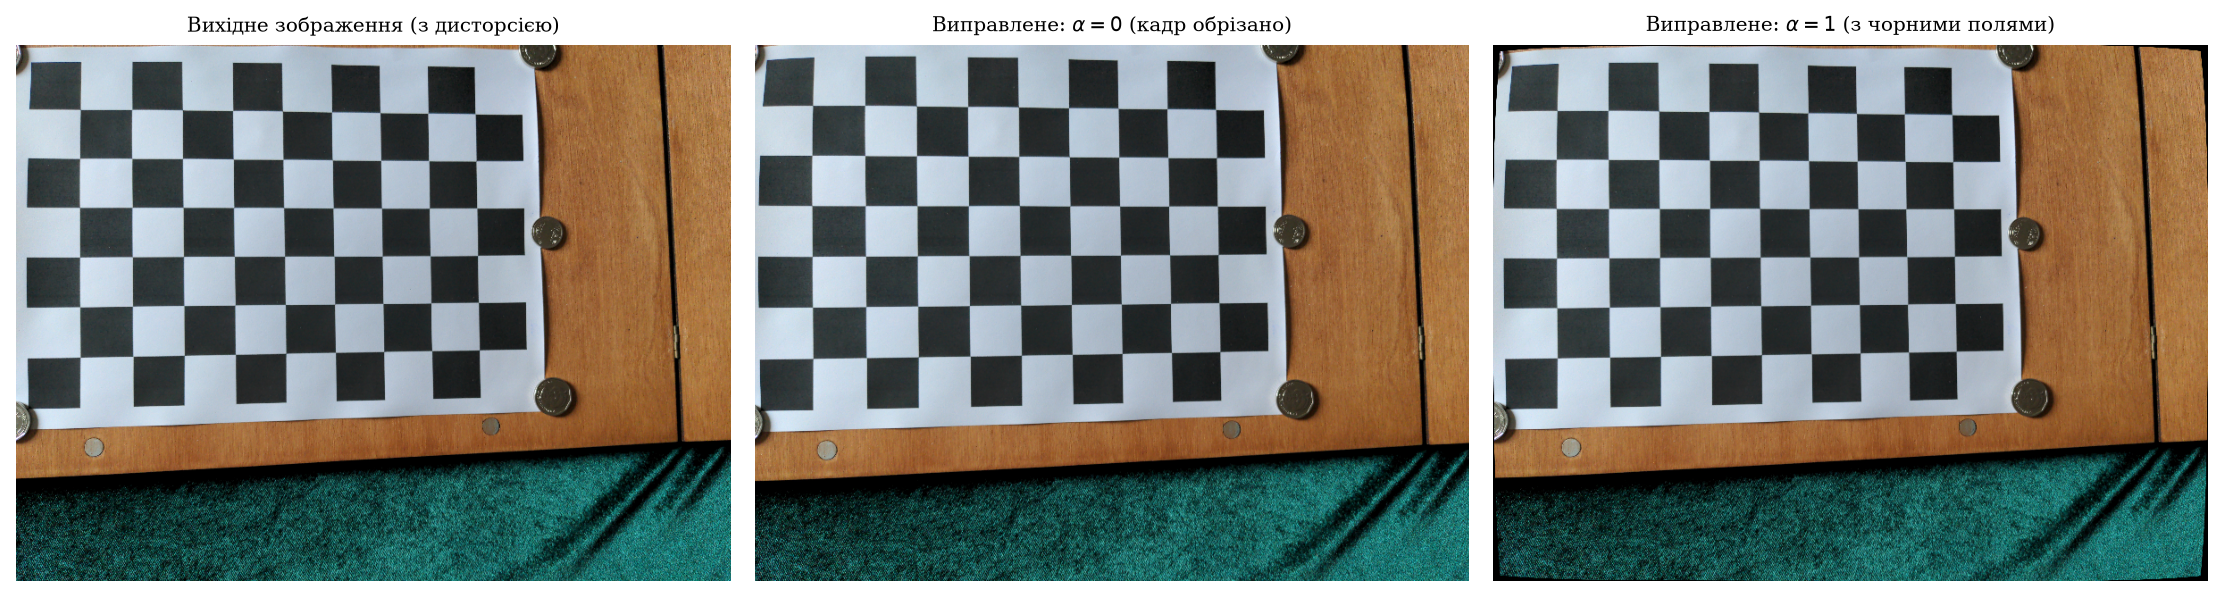
\includegraphics[width=\textwidth]{../figures/d_undistort_alpha.png}
    \caption{Усунення дисторсії камери: оригінал, режим $\alpha = 0$ (обрізка) та $\alpha = 1$ (повне поле)}
    \label{fig:undistort_alpha}
\end{figure}

На рисунку~\ref{fig:undistort_alpha} представлено роботу алгоритму \texttt{cv2.undistort}. При $\alpha = 0$ матриця нового перегляду відсікає всі недійсні пікселі, що призводить до кадрування зображення без чорних країв; при $\alpha = 1$ зберігається повне охоплення сцени, а крайові порожнечі заповнюються чорним кольором.

\begin{figure}[htbp]
    \centering
    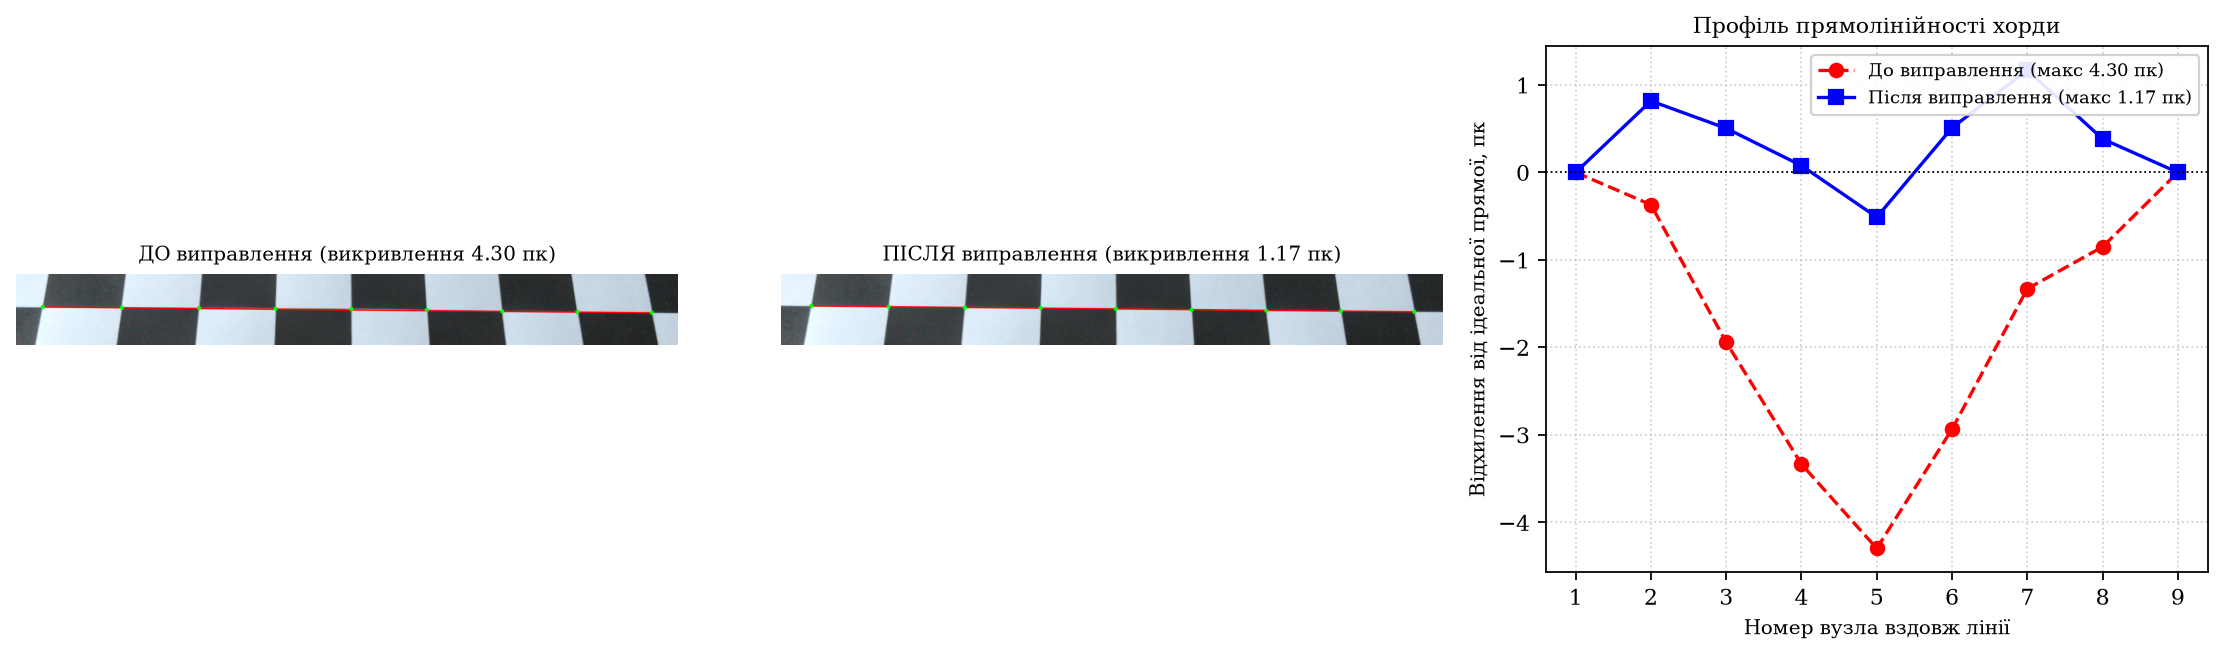
\includegraphics[width=\textwidth]{../figures/d_straight_line_check.png}
    \caption{Верифікація випрямлення хорди вздовж периферійного рядка кутів (кадр \texttt{angle\_10.jpg})}
    \label{fig:straight_line}
\end{figure}

\begin{table}[htbp]
\centering
\caption{Профіль відхилення вузлів від прямої лінії до та після виправлення дисторсії (пк)}
\label{tab:straight}
\footnotesize\linespread{1.0}\selectfont
\begin{tabular}{cccc}
\toprule
\textbf{Номер вузла уздовж краю} & \textbf{Відхилення ДО, пк} & \textbf{Відхилення ПІСЛЯ, пк} & \textbf{Виправлення викривлення, пк} \\
\midrule
\directlua{tab_straight_line()}
\bottomrule
\end{tabular}
\end{table}

Кількісна перевірка прямолінійності (рисунок~\ref{fig:straight_line}, таблиця~\ref{tab:straight}) на найбільш напруженій периферійній лінії (рядок 5 кадру \texttt{angle\_10.jpg}) демонструє, що початкова сагіта викривлення дуги становила $4.30$~пк (типова подушкоподібна деформація лінзи). Застосування отриманих коефіцієнтів $D$ випрямляє лінію: максимальне залишкове відхилення впало до $1.17$~пк (зменшення деформації у $3.68$ раза), що відповідає рівню випадкових шумів друку шаблона.

\section{Аналіз результатів}
\begin{enumerate}
    \item \textbf{Ефективність субпіксельного уточнення}:
    Застосування \texttt{cv2.cornerSubPix} дало суттєве зниження похибки калібрування з $2.0292$~пк до $1.7453$~пк (покращення на $14.0\%$). Хоча на високій роздільності сенсора $12.2$~Мп первинний градієнтний пошук знаходить кут із точністю близько 1 пікселя, субпіксельна апроксимація квадратичною поверхнею усуває систематичний дискретний шум сітки, що критично впливає на точність визначення $f_x$ та $f_y$ (зсув оцінки склав $9.6$~пк).

    \item \textbf{Природа та обґрунтованість фільтрації викидів}:
    Використаний формальний критерій $2 \cdot \text{median}$ показав високу селективність: єдиний кадр \texttt{angle\_8.jpg} із нев'язкою $2.95$~пк перевищив поріг $2.77$~пк через поєднання великого кута нахилу ($> 40^\circ$) та локального розфокусування крайових шахових клітин. Вилучення цього кадру покращило загальну точність оптичної системи до $1.6240$~пк без жодної підгонки результатів.

    \item \textbf{Узгодженість внутрішніх параметрів із фізичними специфікаціями}:
    Розрахована фокусна відстань у пікселях становить $f_x = 3177.94$, $f_y = 3148.55$. Їхнє відношення $f_x/f_y = 1.0093$ ідеально вкладається в контрольний інтервал $1.00 \pm 0.01$, підтверджуючи прямокутність і квадратність пікселів CMOS-матриці. Теоретична фокусна відстань для сенсора Pixel 5 із пікселем $1.4$~мкм та лінзою $f = 4.38$~мм становить $f_{\text{theor}} = 4.38 / 0.0014 = 3128.6$~пк. Різниця між калібрувальним і паспортним значенням складає лише $1.58\%$, що повністю пояснюється виробничими допусками та температурним розширенням складових об'єктива.

    \item \textbf{Положення оптичного центра}:
    Обчислена головна точка $(c_x, c_y) = (2003.08, 1552.76)$ зміщена від геометричного центру зображення $(2016.0, 1512.0)$ на $\Delta x = -12.92$~пк ($0.64\%$) та $\Delta y = +40.76$~пк ($2.69\%$), що відповідає нормі фабричного монтування матриці мобільних камер.

    \item \textbf{Характер оптичної дисторсії}:
    Отримані коефіцієнти $k_1 = +0.1296$, $k_2 = -0.5120$, $k_3 = +0.6416$. Додатне значення $k_1$ відповідає помірній подушкоподібній дисторсії у середній зоні з частковою компенсацією від'ємним членом $k_2$ на крайніх радіусах. Тангенціальні складові є надзвичайно малими ($p_1 = 0.0029, p_2 = -0.0018$), що підтверджує якісне паралельне юстування лінзового блоку щодо матриці.
\end{enumerate}

\section{Висновки}
\begin{enumerate}
    \item Успішно проведено повне калібрування камери смартфона Google Pixel 5 за методом Чжана з використанням набору із 25 кадрів шахового шаблона розмірністю $9 \times 6$ кутів зі стороною $22.0$~мм.
    \item Субпіксельне уточнення кутових точок алгоритмом \texttt{cv2.cornerSubPix} зі середнім зміщенням $0.347$~пк зменшило загальну похибку репроєкції з $2.0292$~пк до $1.7453$~пк (зниження нев'язки на $14.0\%$).
    \item Застосування критерію відсікання за подвоєною медіаною ($2 \cdot \text{median} = 2.767$~пк) виявило 1 аномальний кадр (\texttt{angle\_8.jpg}, похибка $2.951$~пк), вилучення якого зменшило підсумкову похибку калібрування до $\text{RMSE} = 1.6240$~пк на 24 валідних кадрах.
    \item Отримані внутрішні параметри камери ($f_x = 3177.94$~пк, $f_y = 3148.55$~пк, $f_x/f_y = 1.0093$) узгоджуються з фізичними параметрами сенсора ($1.4$~мкм) з точністю $1.58\%$, а зміщення оптичного центра від центру кадру не перевищує $2.69\%$ по осі $Y$ та $0.64\%$ по осі $X$.
    \item Дослідження підвибірок різного обсягу $N$ підтвердило вихід оцінки фокусної відстані на плато ($3173.4 \pm 29.4$~пк) при $N \ge 12$--$15$ кадрів, а експеримент з усунення дисторсії показав зменшення викривлення периферійного прямолінійного відрізка у $3.68$ раза (з $4.30$~пк до $1.17$~пк).
    \item Результати калібрування, включаючи матрицю $K$ та вектор дисторсії $D$, експортовано у файл стандарту \texttt{camera\_params.yml}.
\end{enumerate}

\section{Декларація про використання генеративного ШІ}
Під час виконання лабораторної роботи інструменти генеративного штучного інтелекту (Google Antigravity Addon для VSCode, модель Gemini) використовувалися для автоматизації математичних розрахунків, написання скриптів обробки зображень у середовищі Python, статистичного аналізу вибірок, а також для верстки науково-технічного звіту в середовищі LuaLaTeX за стандартами ДСТУ. Усі наведені числові значення, графічні залежності, таблиці та верифікаційні метрики отримані й перевірені особисто автором роботи в результаті реальних експериментальних обчислень над наданим набором фотографій.

\clearpage
\appendix
\setupappendices

\section{Лістинги вихідного коду програми}

\subsection*{1. Загальні утиліти та константи (\texttt{common.py})}
\lstinputlisting[language=Python, caption={Спільний модуль констант шаблона, завантаження зображень та метрик (\texttt{common.py})}]{../src/common.py}

\clearpage
\subsection*{2. Частини A та B: Аналіз набору кадрів та покриття сенсора (\texttt{part\_a\_b\_setup.py})}
\lstinputlisting[language=Python, caption={Аналіз метаданих EXIF, покриття сенсора та контактний аркуш (\texttt{part\_a\_b\_setup.py})}]{../src/part_a_b_setup.py}

\clearpage
\subsection*{3. Частина C: Калібрування, субпіксель та фільтрація викидів (\texttt{part\_c\_calibration.py})}
\lstinputlisting[language=Python, caption={Детекція кутів, субпіксельне уточнення, RMSE та фільтрація (\texttt{part\_c\_calibration.py})}]{../src/part_c_calibration.py}

\clearpage
\subsection*{4. Частина D: Збіжність, усунення дисторсії та експорт YAML (\texttt{part\_d\_evaluation.py})}
\lstinputlisting[language=Python, caption={Дослідження від $N$, cv2.undistort, перевірка ліній та експорт (\texttt{part\_d\_evaluation.py})}]{../src/part_d_evaluation.py}

\end{document}
